\chapter{Implementation}
\textit{I give the overview of the project repository. I move on to explain the  }

\section{Repository Overview}

\dirtree{%
	.1 P4-NetFPGA.
		.2 project.
			.3 simple\_sume\_switch.
				.4 hw.
					.5 hdl.
						.6 nf\_datapath.v*.
				.4 test.
					.5 sim\_switch\_default.
						.6 run.py*.
			.3 src.
				.4 tcp\_retransmit.p4*.
				.4 commands.txt*.
			.3 testdata.
				.4 gen\_testdata.py*.
				.4 digest\_data.py*.
				.4 sss\_sdnet\_tuples.py*.
			.3 templates.
				.4 externs.
					.5 <externs-name>.
						.6 hdl.
							.7 <externs-name>\_template.v*.
		.2 lib.
			.3 hw.
				.4 contrib.
					.5 cores.
						.6 sss\_cache\_queues\_v1\_0\_0*.
				.4 std.
					.5 cores.
						.6 output\_arbiter\_v1\_0\_0*.
}


This project will work mainly with a NetFPGA SUME board \cite{zilberman2014netfpga}, using P4 programming language. I will be using the P4-NetFPGA workflow, which provides infrastructure to compile P4 programs to NetFPGA \cite{fpga}. Apart from that, everything else will be built from scratch.

\section{Software Implementation}
	\subsection{The Parser}
Parsers are functions that map packets into headers and metadata, written in a state machine style. A parser is defined by:

{\renewcommand{\baselinestretch}{0.8}\small
	\begin{verbatim}
  // Parser Implementation
  @Xilinx_MaxPacketRegion(8192)
  parser TopParser(packet_in b, 
                  out Parsed_packet p, 
                  out user_metadata_t user_metadata,
                  out digest_data_t digest_data,
                  inout sume_metadata_t sume_metadata) {
                  
        /*** state machine description ***/
        
  }
	\end{verbatim}
}
where \texttt{@Xilinx\_MaxPacketRegion(8192)} is Xilinx P4-SDNet's additional annotation for parser/deparser that declares the largest packet size (in bits) the parser/deparser needs to support.

\begin{figure}[h]
	\centering
	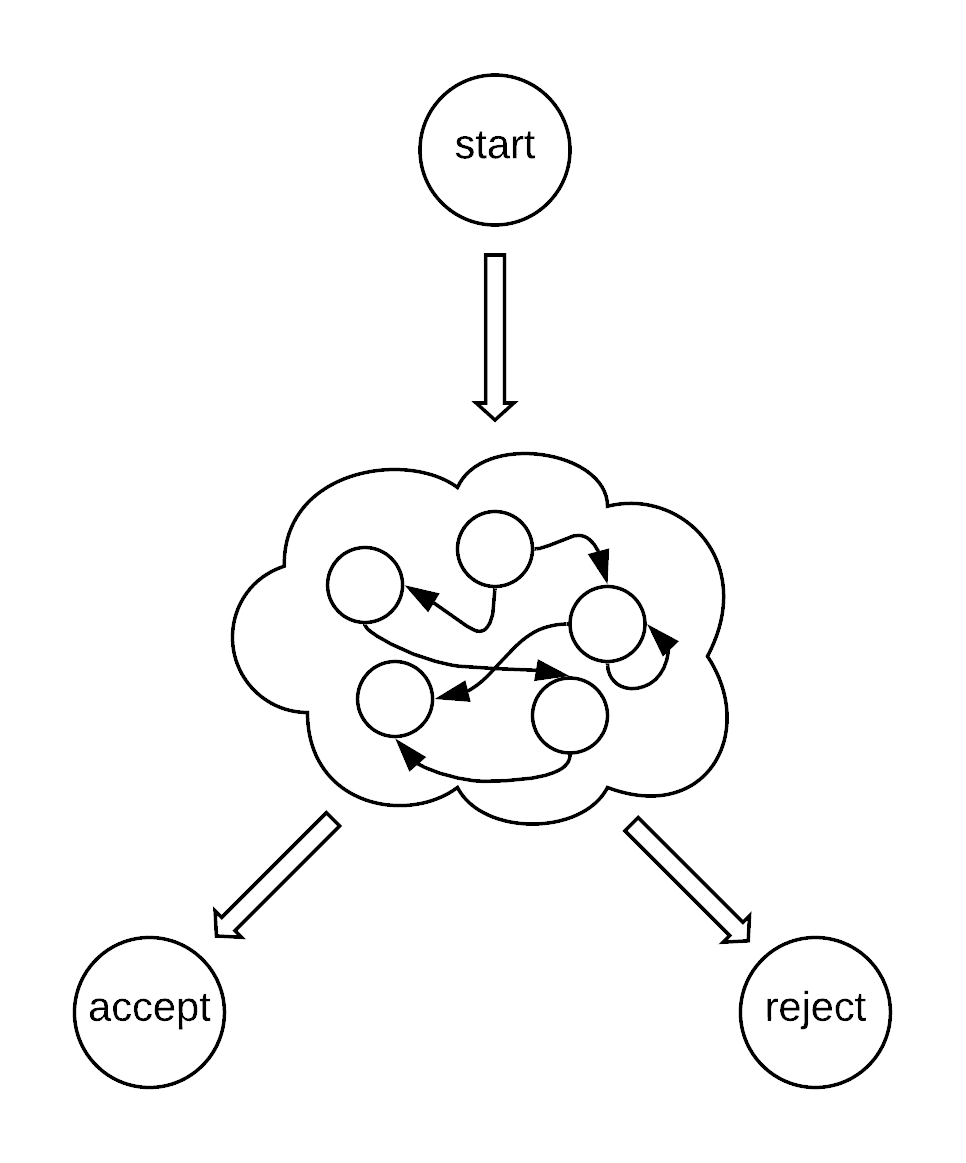
\includegraphics[width=0.4\textwidth]{general-fsm.png}
	\caption{Parser general FSM structure.}
	\label{general-fsm}
\end{figure}
 
Figure \ref{general-fsm} illustrates the general structure of a parser state machine, which includes three predefined states: 
\begin{itemize}
	\item \texttt{start} -- the start state.
	\item \texttt{accept} -- indicating successful parsing.
	\item \texttt{reject} -- indicating a parsing failure.
\end{itemize}
and other internal states that may be defined by the user. The \texttt{start} state is part of the parser, while the \texttt{accept} and \texttt{reject} states are distinct from the user-defined states and are logically outside of the parser. 

An architecture must specify the behaviour when the \texttt{accept} and \texttt{reject} states are reached. For example, an architecture may specify that all packets reaching the \texttt{reject} state are dropped without further processing. Alternatively, it may specify that such packets are passed to the next block after the parser, with intrinsic metadata indicating that the parser reached the \texttt{reject} state, along with the error recorded. The SimpleSumeSwitch architecture adopts the former.

\begin{figure}[h]
	\centering
	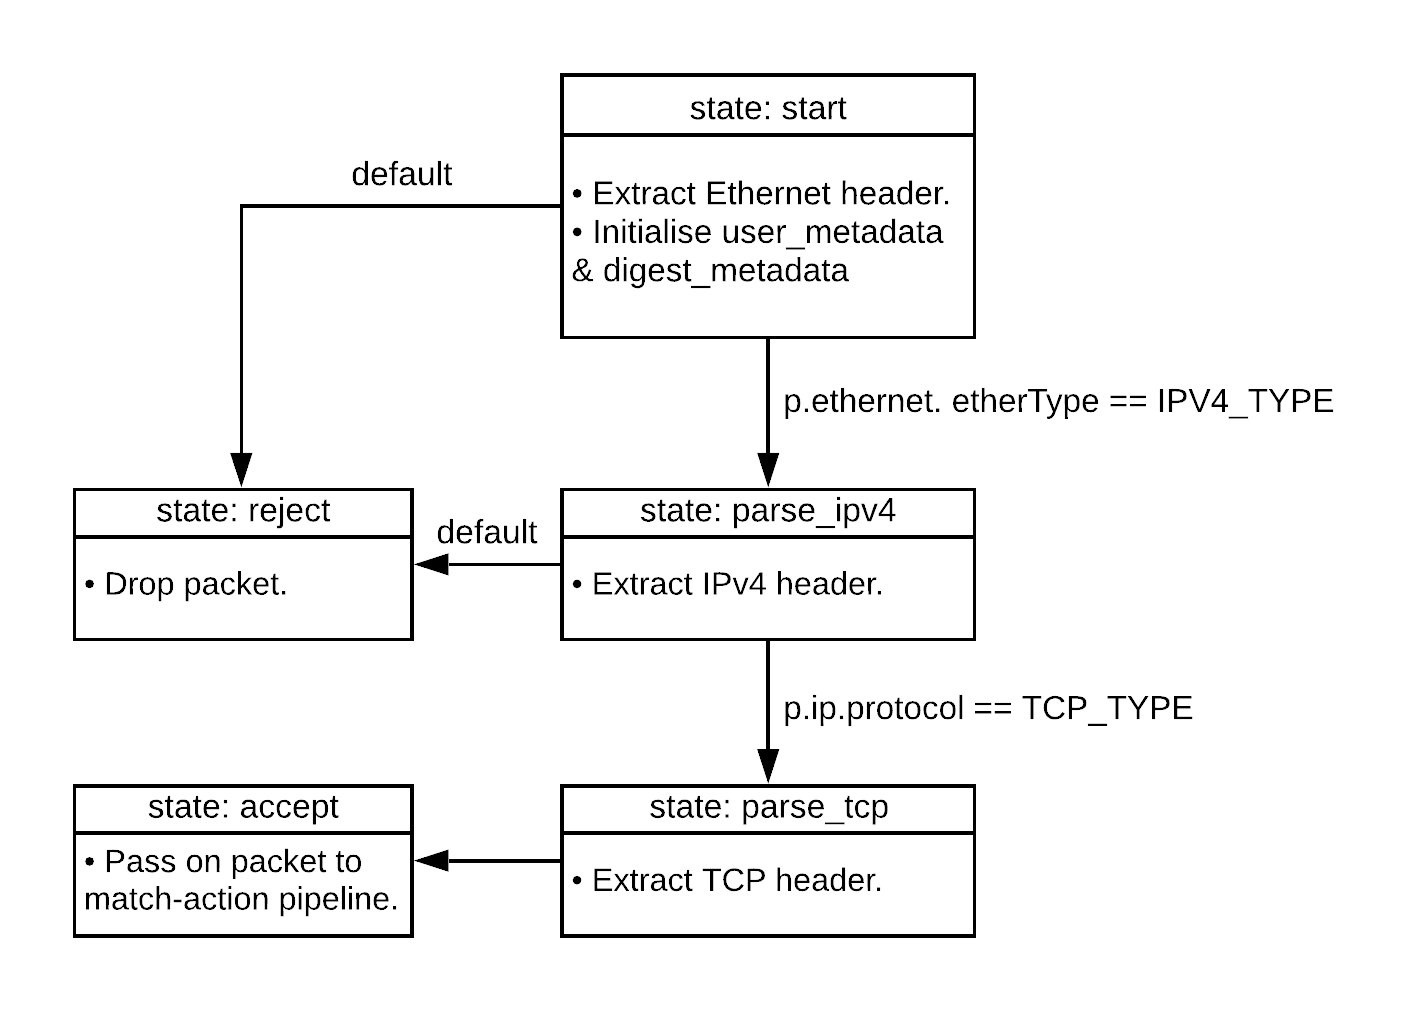
\includegraphics[width=0.8\textwidth]{design-fsm.png}
	\caption{The FSM of the design.}
	\label{design-fsm}
\end{figure}

Figure \ref{design-fsm} describes the FSM structure of my parser, in which I defined two additional states \texttt{parse\_ipv4} and \texttt{parse\_tcp}:

\begin{figure}[!ht]
	\begin{minipage}{.48\textwidth}
		{\renewcommand{\baselinestretch}{0.8}\small
		\begin{verbatim}
		state parse_ipv4 {
		  b.extract(p.ip);
		  transition select(p.ip.protocol) {
		    TCP_TYPE: parse_tcp;
		    default: reject;
		  }
		}
		\end{verbatim}
		}
 		\caption{The definition of \texttt{parse\_ipv4} state.}
	\end{minipage}
	\hfill
	\begin{minipage}{.48\textwidth}
		{\renewcommand{\baselinestretch}{0.8}\small
		\begin{verbatim}
		state parse_tcp {
		  b.extract(p.tcp);
		  transition accept;
		}
		    
		    
		    
		\end{verbatim}
		}	
		\caption{The definition of \texttt{parse\_tcp} state.}
	\end{minipage}
\end{figure}

The P4 \texttt{select} statement is used to branch in a parser. It is similar to \texttt{case} statement in C or Java, but without ``fall-through behaviour''---i.e., \texttt{break} statements are not needed. A \texttt{parse\_ethernet} state could be defined similarly, but I decided to include the parsing of the Ethernet header within the \texttt{start} state, together with initialising the metadata, for simplicity. Here, the \texttt{parse\_ipv4} state extracts the packet's IPv4 header, looks at the \texttt{protocol} field and makes a transition to the \texttt{parse\_tcp} state only if it is \texttt{TCP\_TYPE} which is defined to be 6. Otherwise, the packet is rejected. The \texttt{parse\_tcp} state simply extracts the TCP header of the packet and made a transits to the \texttt{accept} state, where the packet will be passed to the match-action pipeline. 
		
	\subsection{The Match-Action Pipeline}
A match-action pipeline can be defined by the following code sequence:
{\renewcommand{\baselinestretch}{0.8}\small
	\begin{verbatim}
    // Match-action pipeline
    control TopPipe(inout Parsed_packet p,
                  inout sume_metadata_t sume_metadata, 
                  inout digest_data_t digest_data, 
                  inout user_metadata_t user_metadata) {
      /** actions **/
      /** tables **/
      /** logic **/          
    }
	\end{verbatim}
}
This is where the header processing logic is implemented, using a data-dependent sequence of match-action unit invocations and other imperative constructs (indicated by the \textbf{\texttt{control}} keyword). This pipeline receives four inputs: the parsed packet \texttt{p}, the SUME metadata, the digest data and the user metadata. The direction \texttt{inout} indicates that the parameters are both an input and an output. Thus, their values, including the fields in the headers of packet \texttt{p}, can be modified. Nonetheless, the user metadata was not used in this design.

\begin{figure}[!ht]
	\centering
	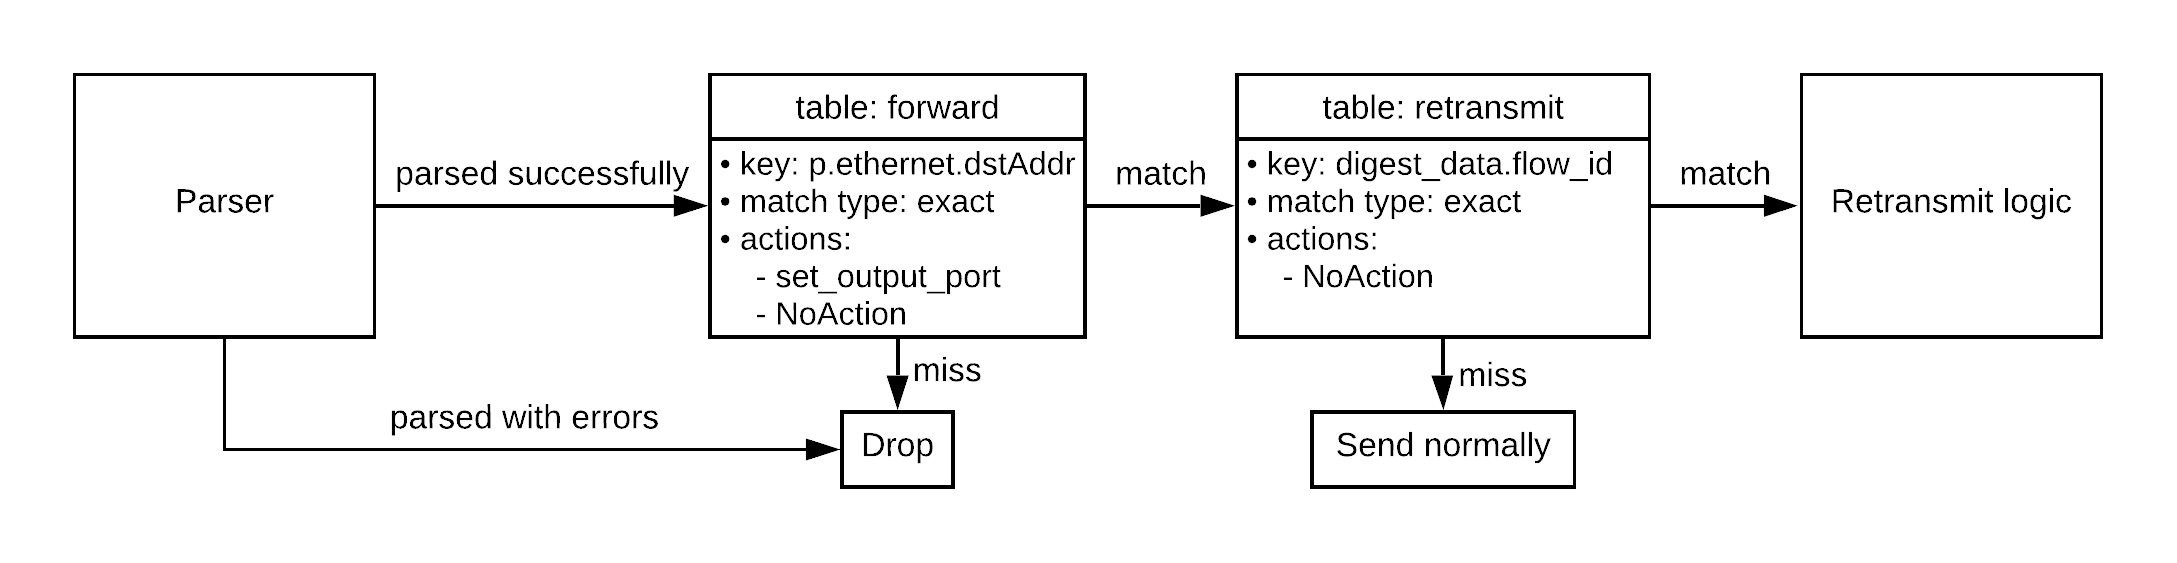
\includegraphics[width=\textwidth]{mapipe.png}
	\caption{A packet processing program describing a simple L2/L3 IPv4 switch.}
	\label{mapipe}
\end{figure}

Figure \ref{mapipe} illustrates the control flow program acting on a packet going through our match-action pipeline, which comprises two match-action units (represented by the P4 \textbf{\texttt{table}} keyword): \texttt{forward} and \texttt{retransmit}.
The first table uses the Ethernet destination address to determine the output port for the next hop. If this lookup fails, the packet is dropped (by assigning \texttt{sume\_metadata.dst\_port} to 0). The second table checks the computed \texttt{digest\_data.flow\_id}: if it matches our flow of interest, the packet will be monitored to assist the fast retransmit of TCP congestion control. Otherwise, the packet will just be sent normally. A packet will be modified by a series of \texttt{action}s: \texttt{set\_output\_port} sets the output port on the SUME board for packets whose Ethernet destination address matches what was defined in the first table, and \texttt{compute\_flow\_id} computes the flow number of the packet for the second table to look up. \texttt{cache\_write}, \texttt{cache\_read} and \texttt{cache\_drop} modify \texttt{digest\_data.tuser} to signal the cache queue to cache, retransmit and drop the packet at the head of the queue respectively.
		
In summary, the switch will perform the following tasks in the SSS module:
\begin{itemize}
	\item Receive and parse packet from the sender.
	\item Look up the Ethernet destination address to determine the output port. Drop on a miss.
	\item Compute the flow number of the packet.
	\item Look up the flow number of the packet to determine if it should be monitored. Send normally on a miss.
	\item Set \texttt{digest\_data.tuser} and/or set the \texttt{ACK} flag in the TCP header appropriately.
	\item Construct the final packet and send it to the receiver.
\end{itemize}

	\subsection{The Deparser}
The inverse of parsing is deparsing, or packet assembly, where the outgoing packet is constructed by reassembling of the headers as computed by the pipeline. P4 does not provide a separate language for packet deparsing; deparsing is done in a \textbf{\texttt{control}} block that has at least one parameter of type \verb|packet_out|. The advantage of this approach is that it makes deparsing explicit, but decouples it from parsing. 

The following code block, which implements the deparser of the switch, first writes an Ethernet header, followed by an IPv4 header, and then a TCP header into a \verb|packet_out|. Since emitting a header appends the header to the \verb|packet_out| only if the header is valid, P4 first checks the validity of the headers before serialising them.

{\renewcommand{\baselinestretch}{0.8}\small
\begin{verbatim}
  // Deparser Implementation
  @Xilinx_MaxPacketRegion(8192)
  control TopDeparser(packet_out b,
                  in Parsed_packet p,
                  in user_metadata_t user_metadata,
                  inout digest_data_t digest_data, 
                  inout sume_metadata_t sume_metadata) { 
      apply {
        b.emit(p.ethernet); 
        b.emit(p.ip);
        b.emit(p.tcp);
      }
  }
\end{verbatim}
}
		
	\subsection{The Externs}
P4 externs are platform-specific functions that are not described in the core P4 language---some sort of ``black boxes'' for P4 programs. They can either be \textbf{stateless}---reinitialised for each packet---or \textbf{stateful}---keeping states between packets. A set of supported externs is defined by the architecture in the \texttt{templates} folder. In this project, the following 

An important feature of P4$\rightarrow$NetFPGA externs is that each stateful atom (i.e. register) can only be accessed \textit{one} time in the P4 code. Multiple calls to the extern function will generate multiple instances of the atom and thus will likely give unexpected results. This complicates my 

\section{Hardware Implementation}
	\subsection{The Cache Queue}
	
	\subsection{The Output Arbiter}
The P4$\rightarrow$NetFPGA platform comes with an input arbiter, which performs the following functions:
\begin{itemize}
	\item It receives packets from one of the physical input Ethernet ports, from the control plane, or from the input recirculation port.
	\item For packets received from Ethernet ports, the block computes the Ethernet trailer checksum and verifies it. If the checksum does not match, the packet is discarded. If the checksum does match, it is removed from the packet payload.
	\item Receiving a packet involves running an arbitration algorithm if multiple packets are available.
	\item If the arbiter block is busy processing a previous packet and no queue space is available, input ports may drop arriving packets, without indicating the fact that the packets were dropped in any way.
	\item 	After receiving a packet, the arbiter block sets the inCtrl.inputPort value that is an input to the match-action pipeline with the identity of the input port where the packet originated. Physical Ethernet ports are numbered 0 to 7, while the input recirculation port has a number 13 and the CPU port has the number 14. 
\end{itemize}
For our architecture, since we have two queues---the output queue and the cache queue---we would require an ``output'' arbiter for each of the five ports.

